\chapter{Classification and regression trees}\label{ch:cart}

\begin{remark}{Outline}
In this chapter, we present a unified framework in which we detail (single)
decision trees methods. In Section~\ref{sec:3:introduction}, we first give an
overview of the context in which these algorithms have been developed. In
Section~\ref{sec:3:tree-structured-models}, we proceed with a mathematical
presentation, introducing all necessary concepts and notations. The general
learning algorithm is then presented in Section~\ref{sec:3:induction} while
more advanced concepts are discussed in finer details in Sections~\ref{sec:3:splitting-rules}
and \ref{sec:3:criteria}. As such, specific algorithms (e.g.,
CART, ID3 or C4.5) are described as specializations of the general framework
presented here.
\end{remark}

\section{Introduction}
\label{sec:3:introduction}

Since always, artificial intelligence has been driven by the ambition to
understand and uncover complex relations in data. That is, to find models that
can not only produce accurate predictions, but also be used to extract
knowledge in an intelligible way. Guided with this twofold objective, research
in machine learning has given rise to extensive bodies works in a myriad of
directions. Among all of them however, tree-based methods stand as one of
the most effective and useful method, capable to produce both reliable and
understandable results, on mostly any kind of data.

Historically, the appearance of \textit{decision trees} is due to
\citet{morgan:1963}, who first proposed a tree-based method called
\textit{automatic interaction dectection} for handling multi-variate
non-additive effects in the context of survey data. Without contest however, the
principal investigators that have driven research on the methodological
principles  are \citet{breiman:1978a,breiman:1978b},
\citet{friedman:1977,friedman:1979} and \citet{quinlan:1979,quinlan:1986} who
simultaneously and independently proposed very close algorithms for the
induction of tree-based models. Most notably, the summarizing work of
\citet{breiman:1984}, later complemented with the work of \citet{quinlan:1993},
have set decision trees into a simple and consistent methodological framework,
which largely contributed in making them easy to understand and easy to use by
a large audience.

As we will explore in further details all throughout this work, the success
of decision trees (and by extension, of all tree-based methods) is explained
by several factors that make them attractive in practice:
\begin{itemize}
\item Decision trees are non-parametric. They can model arbitrarily complex relations between inputs and outputs, without any a priori assumption;
\item Decision trees handle heterogeneous data (ordered or categorical variables, or a mix of both);
\item Decision trees intrinsically implement feature selection, making them robust to irrelevant or noisy variables;
\item Decision trees are robust to outliers or errors in labels;
\item Decision trees are easily interpretable, even for non-statistically oriented users.
\end{itemize}

Most importantly, decision trees are at the foundation of
many modern and state-of-the-art algorithms, including forests of randomized
trees (on which this work is about, see Chapter~\ref{ch:forest}) or
boosting methods~\citep{freund:1995,friedman:2001}, where they are used
as building blocks for composing larger models. Understanding all algorithmic
details of single decision trees is therefore an expected prerequisite
for an in-depth analysis of these methods.


\section{Tree structured models}
\label{sec:3:tree-structured-models}

When the output space is a finite set of values, like in classification where
${\cal Y} = \{c_1, c_2, ..., c_J\}$, another way of looking at a supervised
learning problem is to notice that $Y$ defines a partition over the input space ${\cal X}$, that
is
\begin{equation}
{\cal X} = {\cal X}_{c_1} \cup {\cal X}_{c_2} \cup ... \cup {\cal X}_{c_J},
\end{equation}
where ${\cal X}_{c_k}$ is the set of objects $\mathbf{x}$ for which
$Y$ has value $c_k$. Similarly, a classifier $\varphi$ can also be
regarded as a partition of the input space
${\cal X}$ since it defines an approximation $\widehat{Y}$ of $Y$, which in
turn partitions ${\cal X}$, that is
\begin{equation}\label{eqn:3:partition}
{\cal X} = \widehat{{\cal X}_{c_1}} \cup \widehat{{\cal X}_{c_2}} \cup ... \cup \widehat{{\cal X}_{c_J}},
\end{equation}
where
$\widehat{{\cal X}_{c_k}}$ is the set of objects $\mathbf{x}$ such that
$\varphi(\mathbf{x}) = c_k$. Accordingly, learning a classifier can thus
be restated as learning a partition of ${\cal X}$ matching as closely as
possible the (true) partition engendered by $Y$ over ${\cal X}$.

\begin{remark}{Partitioning with noise}
Notice that when $Y$ cannot be univocally determined given $X=\mathbf{x}$,
e.g., when there is noise on $Y$, then the subsets ${\cal X}_{c_k}$ are not
necessarily disjoints. There may exist two distinct objects from the universe $\Omega$ such
that their representations $\mathbf{x}_1$ and $\mathbf{x}_2$ in the input space
are equal, yet such that the corresponding output values $y_1$ and $y_2$ are unequal.
By contrast, since $\varphi$ defines a function from ${\cal X}$ to ${\cal Y}$,
any input $\mathbf{x} \in {\cal X}$ is mapped to exactly one output value $y \in
{\cal Y}$ and the subsets $\widehat{{\cal X}_{c_k}}$ are therefore necessarily
disjoints, which means that no model will ever perfectly predict the true output
value in all cases. As discussed in Section~\ref{sec:2:bayes-model}, this
limitation is unavoidable and can in fact be viewed as the cause of the residual error.
\end{remark}

From a geometrical point of view, the principle of tree structured models is
beautifully simple. It consists in recursively partitioning the input space
${\cal X}$ into subspaces and then assign constant prediction values
$\widehat{y}\in{\cal Y}$ to all objects $\mathbf{x}$ within each terminal
subspace. To make things clearer, let us first define the following concepts:

\begin{definition}
A \emph{tree} is a graph $G=(V,E)$ in which any two vertices (or \emph{nodes})
are connected by exactly one path.
\end{definition}

\begin{definition}
A \emph{rooted tree} is a tree in which one of the nodes has been designated as
the \emph{root}. In our case, we additionally assume that a rooted tree is a
\emph{directed} graph, where all edges are directed away from the root.
\end{definition}

\begin{definition}
If there exists an edge from $t_1$ to $t_2$ (i.e., if $(t_1, t_2)\in E$) then
node $t_1$ is said to be the \emph{parent} of node $t_2$ while node $t_2$ is
said to be a \emph{child} of node $t_1$.
\end{definition}

\begin{definition}
In a rooted tree, a node is said to be \emph{internal} if it has one or more
children and \emph{terminal} if it has no children. Terminal nodes are also
known as \emph{leaves}.
\end{definition}

\begin{definition}
A \emph{binary tree} is a rooted tree where all internal nodes exactly
have two children.
\end{definition}

In those terms, a \textit{tree-structured model} (or \textit{decision tree})
can be defined as a model $\varphi: {\cal X} \mapsto {\cal Y}$ represented by a
rooted tree (often binary, but not necessarily), where any node $t$ represents
a subspace ${\cal X}_t \subseteq {\cal X}$ of the intput space, with the root
node corresponding to ${\cal X}$ itself. Internal nodes $t$ are labeled with a
\textit{split} $s_t$ (taken from a set of questions ${\cal Q}$) dividing the
space ${\cal X}_t$ they each represent into disjoint subspaces respectively
corresponding to each of their children. For instance, the set of all binary
splits is the set ${\cal Q}$ of questions $s$ of the form \textit{``Is
$\mathbf{x} \in {\cal X}_A?$''}, where ${\cal X}_A \subset {\cal X}$ is some
subset of the input space. Any split $s$ of this form divides ${\cal X}_t$ into
two subspaces respectively corresponding to ${\cal X}_t \cap {\cal X}_A$ for
the left child of $t$ and to ${\cal X}_t \cap ({\cal X}\setminus{\cal X}_A)$
for the right child of $t$. Terminal nodes are labeled with a best guess value
$\widehat{y}_t \in {\cal Y}$ of the output variable. If $\varphi$ is a
classification tree, then $\widehat{y}_t \in \{ c_1, ..., c_J \}$ while if
$\varphi$ is a regression tree, then $\widehat{y}_t \in \mathbb{R}$. As such,
the predicted output value $\varphi(\mathbf{x})$ for some instance $\mathbf{x}$
is the label of the leaf reached by the instance when it is propagated through
the tree by following the splits $s_t$.

\begin{remark}{Induction graphs}
From a graph theory point of view, decision trees belong to a larger family
of methods known as \textit{induction graphs}~\citep{zighed:2000}. In this more
general framework, the structure is a directed acyclic graph, which allows for
nodes to be both divided and recombined.
\end{remark}

\begin{figure}
    \centering
    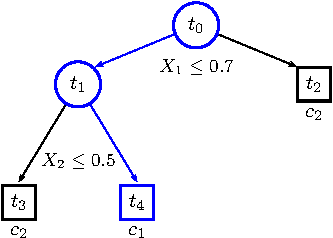
\includegraphics[scale=1.0]{figures/ch3_tree.pdf}
    \caption{A decision tree $\varphi$ built for a binary classification
             problem from an input space ${\cal X}=[0,1]\times[0,1]$.
             (Figure inspired from \citet{breiman:1984}.)}
    \label{fig:3:tree}
\end{figure}

As an example, Figure~\ref{fig:3:tree} illustrates a decision tree $\varphi$
made of five nodes and partitioning the input space ${\cal X} = {\cal X}_1
\times {\cal X}_2 = [0;1] \times [0; 1]$ for a binary classification problem
(where ${\cal Y}=\{ c_1, c_2 \}$). Node $t_0$ is the root node and corresponds
to the whole input space ${\cal X}_{t_0} = {\cal X}$. It is labeled with the binary
split $X_1 \leq 0.7$ (i.e., the question \textit{``Is $X_1 \leq 0.7$?''}) which divides ${\cal X}_{t_0}$ into two disjoint subsets
${\cal X}_{t_1} \cup {\cal X}_{t_2}$. The first set corresponds to its left
child $t_1$ and represents the set of all input vectors $\mathbf{x} \in {\cal
X}_0$ such that $x_1 \leq 0.7$. Similarly, the second set corresponds to its
right child $t_2$ and represents the set of all input vectors $\mathbf{x} \in
{\cal X}_{t_0}$ such that $x_1 > 0.7$. Likewise, $t_1$ is labeled with the
split $X_2 \leq 0.5$ which further divides ${\cal X}_{t_1}$ into two disjoint
subsets ${\cal X}_{t_3} \cup {\cal X}_{t_4}$ respectively corresponding the
sets of all input vectors $\mathbf{x} \in {\cal X}_{t_1}$ such that $x_2 \leq
0.5$ (resp. $x_2 > 0.5$). Terminal nodes $t_2$, $t_3$ and $t_4$ are represented
by squares labeled with an output value $\widehat{y}_t$. They form together a
partition (as defined by Equation~\ref{eqn:3:partition}) of ${\cal X}$, where
each set $\widehat{{\cal X}_{c_k}}$ is obtained from the union of the subspaces
${\cal X}_t$ of all terminal nodes $t$ such that $\widehat{y}_t = c_k$. In this
case, $\widehat{{\cal X}_{c_1}} = {\cal X}_{t_4}$ while $\widehat{{\cal
X}_{c_2}} = {\cal X}_{t_2} \cup {\cal X}_{t_3}$. As shown in
Figure~\ref{fig:3:partition}, the partition engendered by  $\varphi$ on ${\cal
X}$ divides the input space into subspaces that are more and more class
homogeneous, starting from ${\cal X}$ at the root node,  then ${\cal X}_{t_1}
\cup {\cal X}_{t_2}$ at the second level of tree and finally $({\cal X}_{t_3}
\cup {\cal X}_{t_4})\cup {\cal X}_{t_2}$ at the leaves.  As we will explore in
Section~\ref{sec:3:splitting-rules}, the partition is in this case made of
rectangles because of the nature of the splits $s_t \in {\cal Q}$ dividing the nodes.
Predictions are made by propagating instances through the tree and using as
output value the value labeling the terminal nodes in which they fall
into. For example, an object $\mathbf{x}=(x_1=0.2, x_2=0.7)$ falls into $t_4$
and therefore $\varphi(\mathbf{x}) = \widehat{y}(t_4) = c_1$.

\begin{figure}
    \centering
    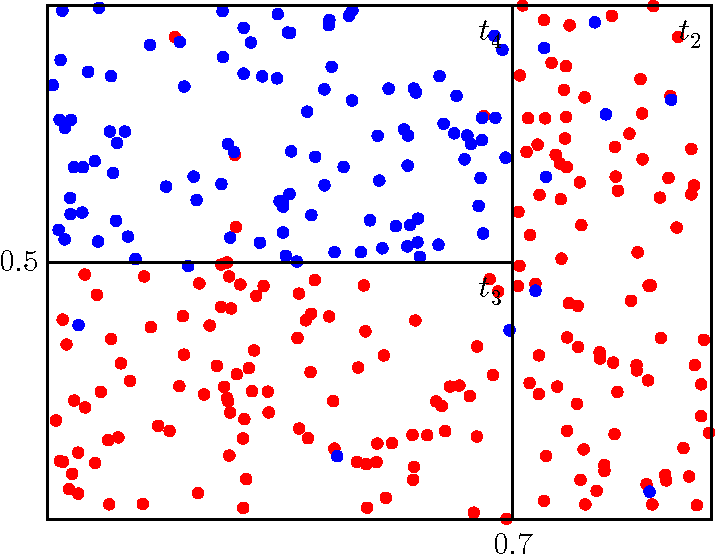
\includegraphics[scale=0.5]{figures/ch3_partition.pdf}
    \caption{Partition of ${\cal X}$ induced by the decision tree $\varphi$.
             Blue dots correspond to objects of class $c_1$ while red dots correspond
             to objects of class $c_2$. (Figure inspired from \citet{breiman:1984}.)}
    \label{fig:3:partition}
\end{figure}


\section{Induction of decision trees}
\label{sec:3:induction}

Learning a decision tree ideally amounts to determine the tree structure which
produces the partition which is closest to the partition engendered by $Y$ over
${\cal X}$. Since it is unknown, the construction of a decision tree is usually
driven instead with the objective of finding a model which explains the
learning set ${\cal L}$ as best as possible. Among all decision trees $\varphi
\in {\cal H}$ however, there may exist several of them that explain ${\cal L}$
equally best. Following Occam's Razzor principles of prefering the explanation
which makes as few assumptions as possible, that is to favor the simplest
solution that fits the data, learning a decision tree from ${\cal L}$ is then
usually restated as finding the smallest tree $\varphi^*$ minimizing its
resubstitution estimate $\overline{E}(\varphi^*, {\cal L})$. While this
assumption makes sense from a generalization point of view, it also makes
sense regarding interpretability. A decision tree which is small is easier
to understand than a large and complex tree.

As shown by \citet{hyafil:1976} however, finding the smallest tree $\varphi^*$
that minimizes its resubstitution estimate is a NP-complete problem. As a
consequence, under the assumption that $P \neq NP$, there exists no efficient
algorithm for finding $\varphi^*$, thereby suggesting that finding efficient heuristics
for constructing near-optimal decision trees is the best solution to keep computation
requirements within realistic boundaries.

As such, decision trees are commonly built using a greedy approach, starting
from a single node and then recursively partitioning the space it represents
into smaller subspaces until convergence.  The learning procedure then revolves
around three elements:

\begin{enumerate}
\item The selection of the splits $s_t \in {\cal Q}$ dividing internal nodes;
\item The choice of a stopping criterion for deciding when a node becomes a terminal node;
\item The assignment of values to terminal nodes.
\end{enumerate}

As we will see, assigning values to terminal nodes happens to be quite simple.
The crux of the problem is in finding good splits and in knowing when to
stop splitting.

% il y a plus d'un decision tree permettant d'expliquer L
% une hypothèse est de considérer le plus simple d'entre eux (occam's razzor comme guide) => prefer the simplest solution that fits the data, pour espérer une bonne généralisation mais aussi une meilleure interprétabilité
% occam : http://fr.slideshare.net/cnu/machine-learning-lecture-3 32
% on pourrait chercher cet arbre en brute force, mais l'espace des arbres est large (quoique fini)
% et en plus c'est NP complet : Constructing Optimal Binary Decision Trees is NP-complete \ref
% (optimal = smallest to explain L)
% => approche greedy/heuristic for near-optimal decision trees are the best solution (sous l'hypothèse P!=NP) pour éviter trop de computations

\subsection{Recursive partitioning}

%  Description de l'algo (high-level)
%       * Recursive partition
%           Depth/Breadth/Best first
%       * Splitting rules (overview)
%           def impurity
%           def decrease impurity
%       * Criterion (overview)

\subsection{Stopping criteria}

%       * Critères d'arrêts [ différents paramètres, chi² ]

\subsection{Assigning values to terminal nodes}

%       * Assignment in terminal nodes, cart 34+

\subsection{Data structures and implementation considerations}

Implementing decision trees involves many issues that are easily overlooked if
not considered with care. The first of these issues concerns the choice of the
data structure for representing decision trees.

Among all possible ways of representing a tree, one of the simplest and most
direct representation is to adopt an object-oriented approach. In this
paradigm, a decision tree is naturally represented as a hierarchy of high-level
objects, where each object corresponds to a node of the tree and comprises
attributes referencing its children or storing its split and value. Such a
representation would make for a correct, intuitive and flexible implementation
but may in fact not be the most appropriate when aiming for high-performance.
One of the biggest issues indeed is that object-oriented programming usually
fragments complex and nested objects into non-contiguous memory blocks, thereby
requiring multiple levels of indirection for traversing the structure. In
particular, this design can easily impair computing times in
performance-critical applications (see Chapter~\ref{ch:complexity} for
benchmarks), e.g., by not making it possible to leverage CPU cache or pre-
fetching mechanisms.

At the price of less abstraction and flexibility, we adopt instead in this work
a low-level representation of decision trees, allowing us for a fine-grained
and complete control over memory management and CPU mechanisms. The tree
representation that we consider ...

%     > Data structures (arrays vs. object-oriented structures)
%       binary vs n-ary tree
%     > définir l'algo de construction
%     > definir l'algo de prédiction


\section{Splitting rules}
\label{sec:3:splitting-rules}

%     > Splitting nodes
%         [ max_features, min_samples_leaf ]
%         - set of questions / answers
%               + categorical vs continuous)
%               + bi-partitions vs n-partitions
%               + weak learners
%         - Best splits
%             + Greedy approximation of optimal trees
%             + optimizing locally the impurity <=> optimizing globally? see page 33+
%         - Approximately best splits
%             + Binning
%             + Subsampling

\section{Goodness of split}
\label{sec:3:criteria}

%     > Impurity criteria
%         - Gini, Entropy, Variance, Information gain etc (see cart + graphes)
%         - Efficient implementation for iterative evaluation
%             + How to evaluate multiple candidate thresholds cheaply for
%               a given feature (algorithm, f-ordered)
%             + Sorting algorithms
%         - Effet du critère sur les cuts
%             End-cut preference (CART 11.8)
%             Normalisation par l'entropy (cf. Vincent, Louis)
%             Effet sur la structure des arbres générés
%         - Sample weighting
%             Negative weights? (@ndawe)

% \section{Interpreting decision trees}
% % From trees to rules
